\chapter{Preliminary Results}

We developed a six-step adopt approach for sidewalk segmentation. 
With the input \ac{VHR} imagery, we locate the sidewalk geometric information and it's initial trajectory, then we generate ribbon image on each sidewalk which has been locate in the map data. 
After that, we adopt density estimation on each pixel in the ribbon image. 
We apply the dynamic programming algorithm with fully developed penalty function to get precious boundaries on sidewalks, then just simply converted the ribbon image back to it's original shape.

\section{Validate Initial Trajectory}

\begin{figure}[H]
    \centering
    \includegraphics[width=\textwidth]{Figures/arizon_center.png}
    \caption[Demonstration on Arizona Center]{Detail demonstration on part of Arizona center, all sidewalks' \ac{GIS} information shows in Orange.}
    \label{fig:arizon_center}
\end{figure}

Before applying deep learning network to determine sidewalk's location, it's necessary to hand marking all sidewalk from imagery or extract the geometric information of each sidewalk from resources like \ac{OSM}. 
It's challenging since the geometric accuracy was not precise, which could cause performance issue since we rely on this information to segment the sidewalk part from maps for the next step. 
To ensure data accuracy, as shows in figure \ref{fig:arizon_center}, we spent days marking all sidewalks and their precise boundaries in Arizona Central for initial experiments. 
We can locate each sidewalk by using the geometric information and saved them into separate files. 
We also calculate the average sidewalk width from boundaries to decide reasonable window size in the following step.

\section{Ribbon Image Generation}

To apply the hypothesis, we develop a way to convert the given sidewalk into a ribbon image. 
As shown in figure \ref{fig:StraightenProcess}, we use the previous outcome (A) from the last step as input and connected all coordinate points data as the mid-line for the sample sidewalk. 
Then we apply a smooth function that we created to smooth the mid-line, so the shape of mid-line fits better to the actual sidewalk shape(B). 
We generate two parallel line as offsets on each side of the mid-line with a distance of twice the average width in between. 
Ideally even the mid-line is not perfectly laying on the middle, we would still fit the whole sidewalk into the ribbon image. 
For each point on the mid-line, we connect the corresponding points on both offsets to get the movement of the sidewalk and recorded them(C, D), we generate the straightened ribbon image by using the color data from each pixel in the points set that we record earlier(E). 
The image data in between each offset, with constant image width could be retrieved after that (F).
Then we reshape the image data to generate the ribbon image(G). 
Figure \ref{fig:Sample_Sidewalk_2} shows the complete ribbon-image output result on sample sidewalk. We separate it into parts to show better detail. 

\begin{figure}[H]
    \centering
    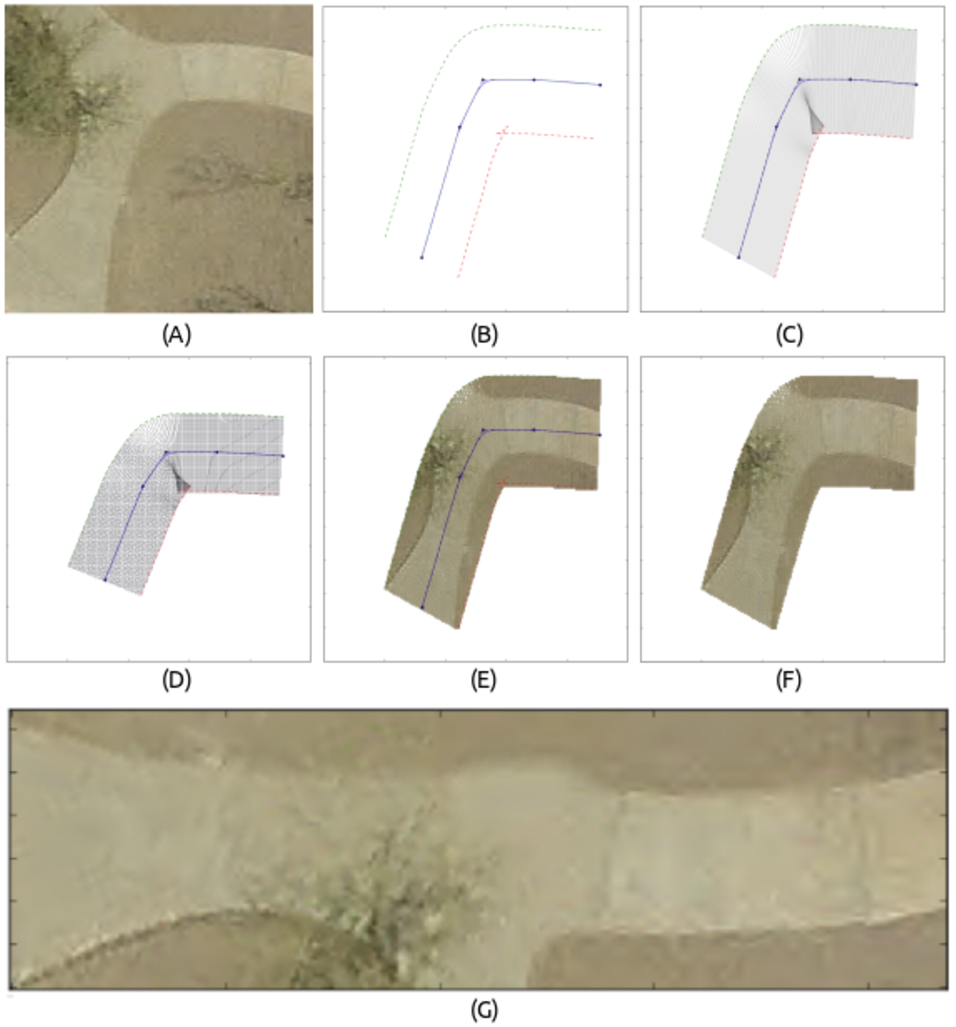
\includegraphics[width=\textwidth]{Figures/straghten.pdf}
    \caption[Ribbon Image Generation]{Ribbon image generating process: from sub-figures A to G, we showed the step by step process to generate ribbon-image from a partial sidewalk. From raw input (A), we smoothed mid line and generated parallel off-site (B). Generated pixels (C) and connected each pixel to its correspond color data from the raw input (D). After gathered pixel data (E), we removed mid-line (F) and generated the ribbon image(G).}
    \label{fig:StraightenProcess}
\end{figure}

\begin{figure}
    \centering
    \includegraphics[width=0.95\textwidth]{Figures/sample2_demo.png}
    \caption[Sample Sidewalk 2]{A ribbon image straighten output on sample sidewalk, row 1 shows the original input, row 2 to 5 show the ribbon image output separate into parts.}
    \label{fig:Sample_Sidewalk_2}
\end{figure}


\section{Density Estimation on Pixels}

Before move on to dynamic programming algorithm, we need to give each pixels a initial score for classification, to classify each pixel is sidewalk or not. 
To achieve that, as shows in figure \ref{fig:GMM_Sample_2}, we applied a density estimation function to find the probability for each pixel in the ribbon image. 
For foreground density, we used grey-scale to determine the probability likely-hood for the sidewalk-feature, where white is more likely to be sidewalk and black is less likely. 
The background density is the opposite, which made black is more likely to be sidewalk and white is not. 
We use the log likely-hood function to calculate the foreground and background density and estimate density on pixels.

\begin{figure}[H]
    \centering
    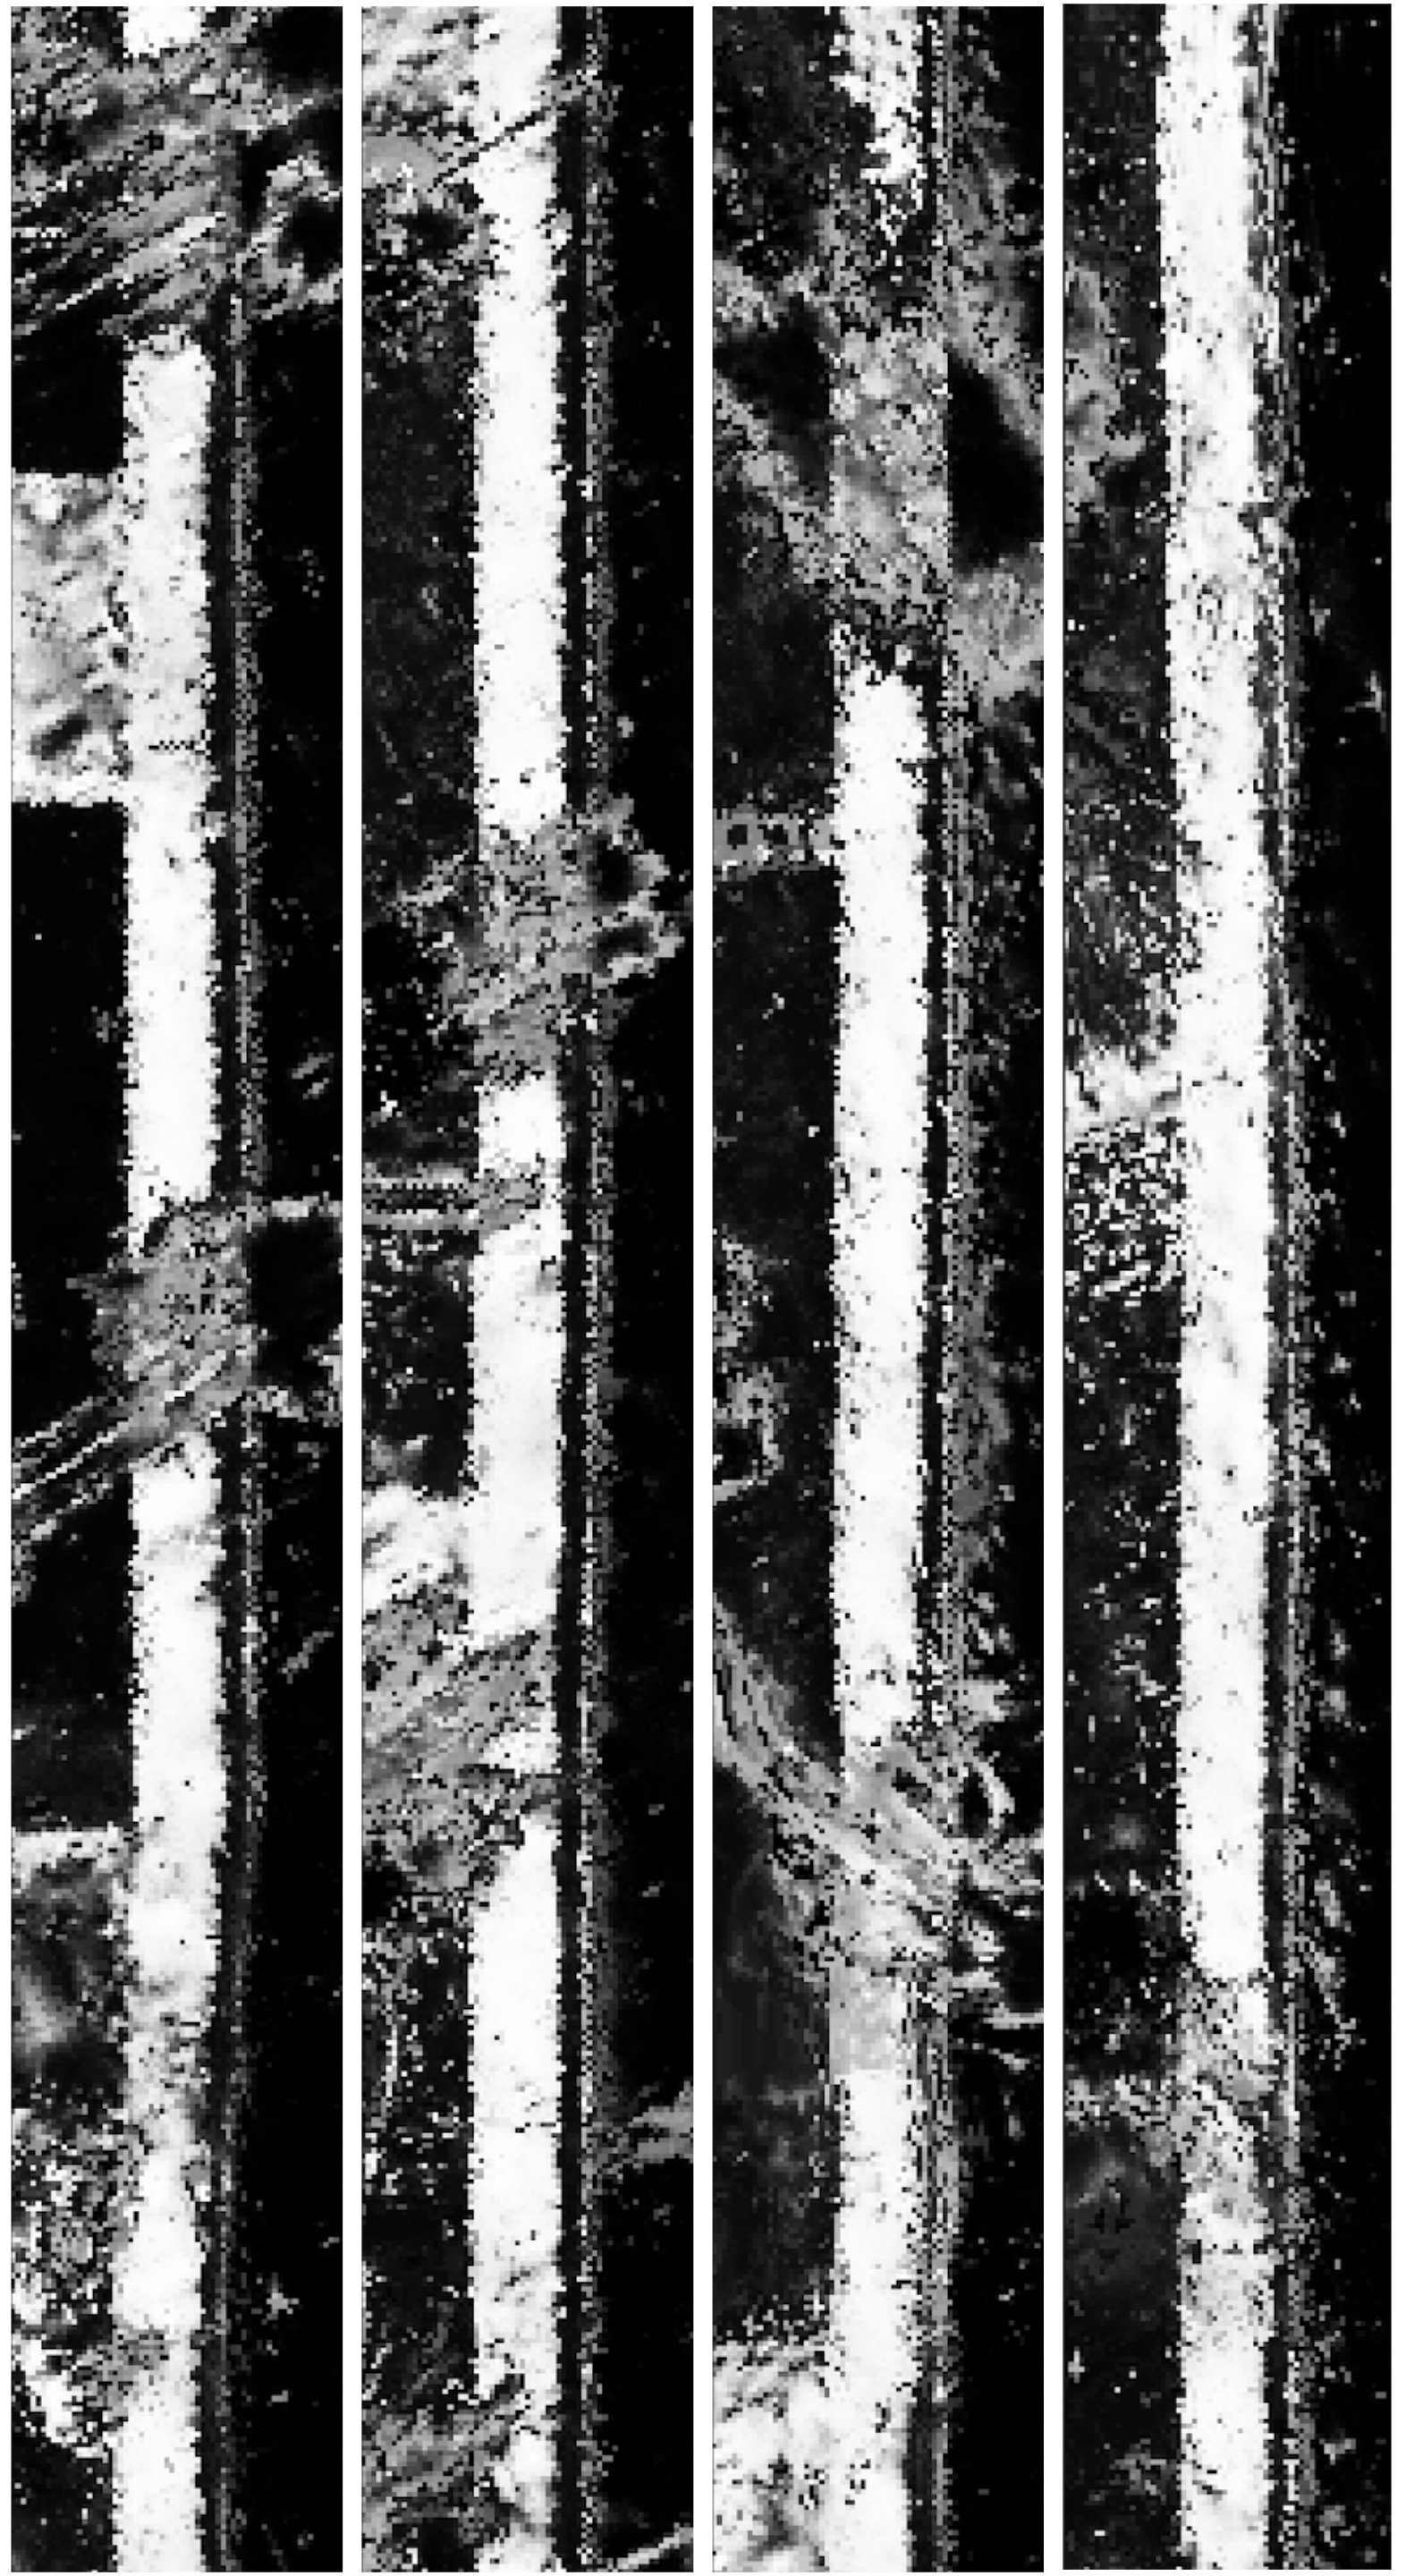
\includegraphics[width=\textwidth]{Figures/GMM_SAMPLE2.png}
    \caption[Density Estimation on Sample Sidewalk]{A sample figure with density estimation applied on figure \ref{fig:Sample_Sidewalk_2}. Where white indicates pixels are more likely to be a sidewalk feature and black indicates pixels are more likely to be a non-sidewalk feature. We separate it into 4 parts from column 1 to 4.}
    \label{fig:GMM_Sample_2}
\end{figure}

\section{The Dynamic Programming Algorithm}

We use our dynamic programming algorithm on the ribbon image to find the max score for each pixel that had better probability to be sidewalk feature that we mentioned in Chapter 4. 
More importantly, we introduce a penalty control function that makes each horizontal movement in the edges or center cost more than vertical movement. Basically, for each line of pixels, if they think the edges or center should shift more horizontally than one pixel compares to the last line, we score them with more penalty. 

Figure \ref{fig:penalty} shows our algorithm managed to separate the driveway and sidewalk under the same feature as penalty increase. So we could apply the dynamic programming solution to locate the precise boundaries of given ribbon image. The penalty control improved our performance significantly. Because of this, our approach could predict the sidewalk under the tree shadow and other shadows or obstacles, which bring us more accurate result compare to other methods.
\begin{figure}[H]
    \centering
    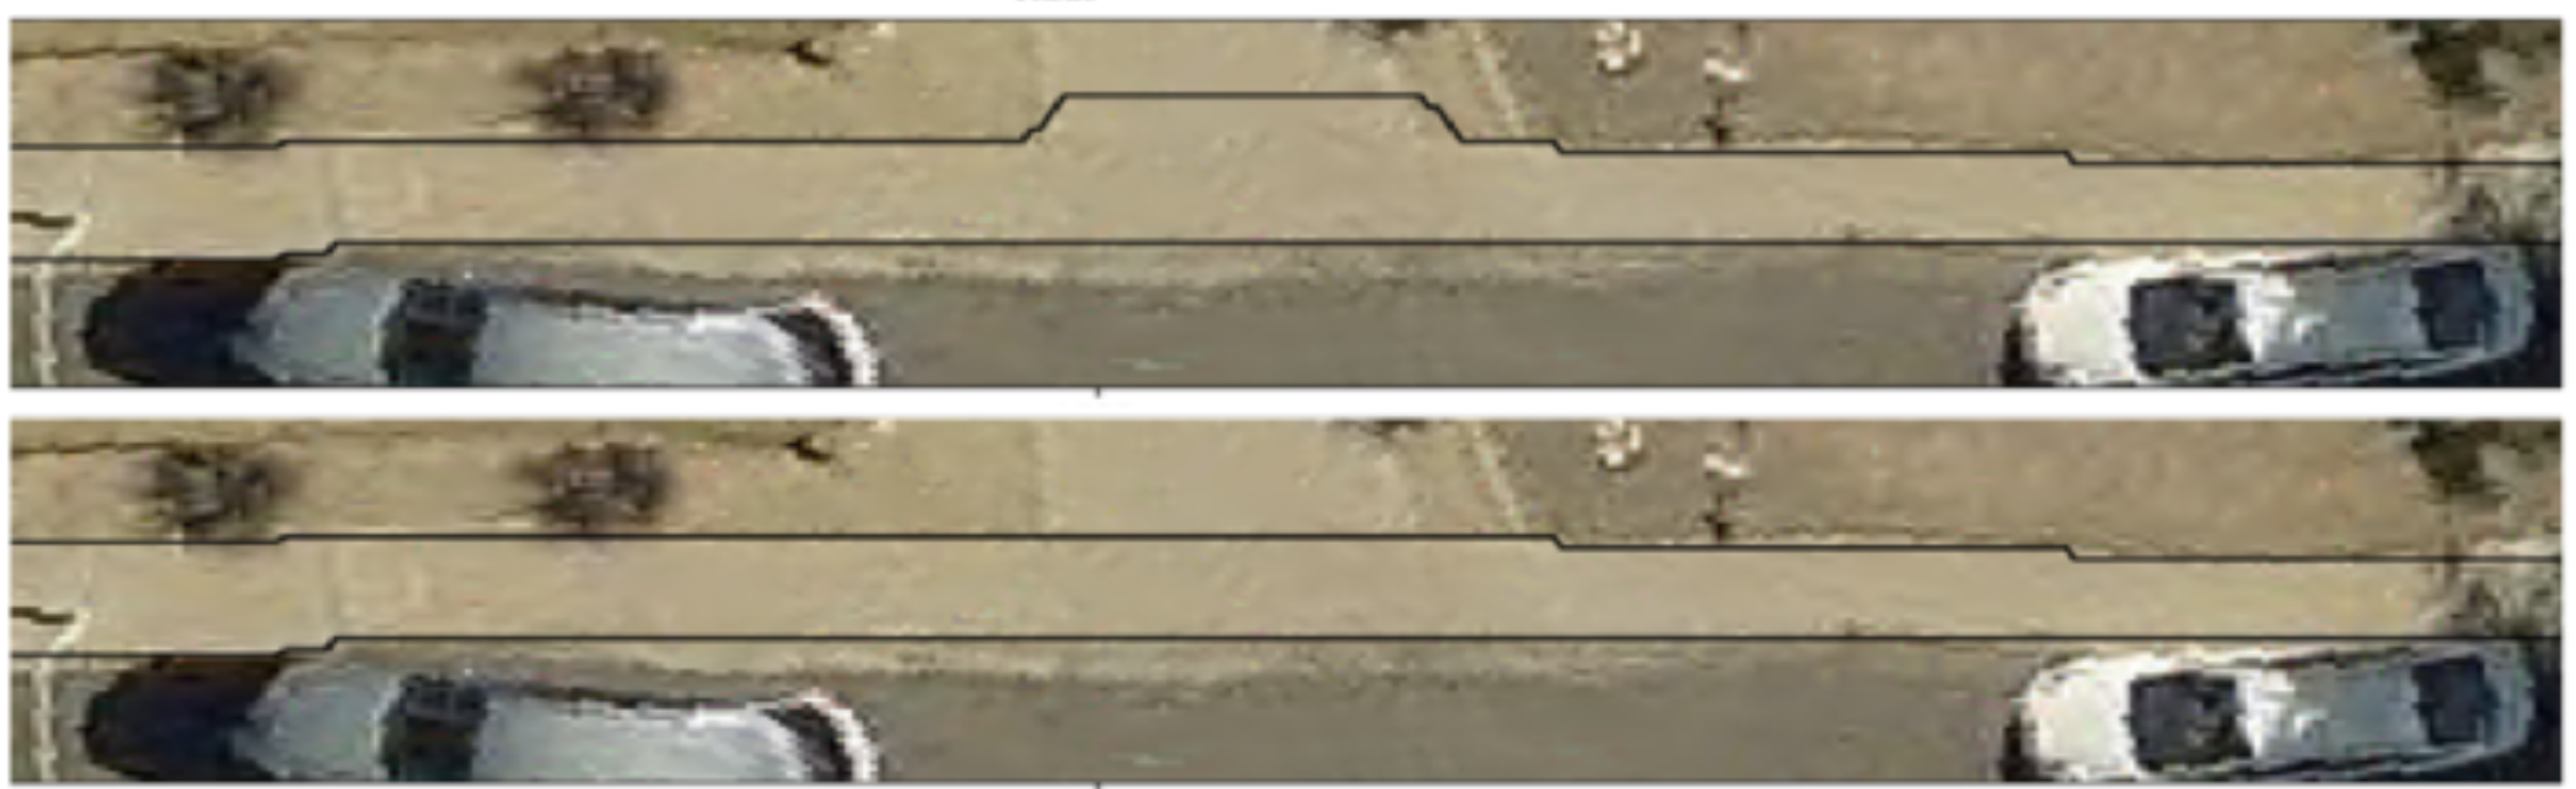
\includegraphics[width=\textwidth]{Figures/penalty.png}
    \caption[Penalty Process]{Comparison with penalty change, we tested a variety of variables to decide which variable had best performance for width control. With the penalty increased at a reasonable amount, our algorithm decided not to recognize a driveway as sidewalk walk, in order to keep the sidewalk width consistent, even though they are the same texture.}
    \label{fig:penalty}
\end{figure}

As shown in figure \ref{fig:sample_result2}, after we generate the result on ribbon image, just need to simply covert the ribbon image back to its original shape by reverse the method that generates the ribbon image. 

\begin{figure}[H]
    \centering
    \includegraphics[width=0.95\textwidth]{Figures/sample2_result.png}
    \caption[Desire Output on Sample Sidewalk]{Detail demonstration on desire result after applying our dynamic programming approach. Where row 1 shows the result after reshape, row 2 to 5 shows the boundaries we calculated on ribbon image from \ref{fig:Sample_Sidewalk_2}.}
    \label{fig:sample_result2}
\end{figure}

\section{Result Evaluation}

We evaluate our results using precision ($P$), recall ($R$) and the balanced F-measure ($F_1$) defined as follows:
\begin{align}
     P &= \frac{\mathit{TP}}{\mathit{TP} + \mathit{FP}}, \\
     R &= \frac{\mathit{TP}}{\mathit{TP} + \mathit{FN}}, \\  
     F_1 &= \frac{2 P R}{P + R}
\end{align}
where 
\acp{TP} is the number of pixels correctly marked as positive, 
\acp{FN} is the number incorrectly marked as negative and 
\acp{FP} is the number incorrectly marked as positive. 

We compare our results against common segmentation approaches 
\ac{SLIC}~\cite{Achanta:149300}, \ActiveContours{}~\cite{ActiveContou09} and \GrabCut{}~\cite{Rother2004-ou} 
in Table~\ref{tab:quantitative-against-common} using a manually annotated region of 
Phoenix AZ. The test region was acquired as \ac{VHR} 4-inch aerial orthophotos, 
and manually annotated by drawing a polygonal outline. 
When a portion of the sidewalk was occluded or camouflage with the surrounding pavement 
(including gutters) we used our best judgment to connect the visible portions of the sidewalk. For all of of the examples we present, with figure \ref{fig:change_on_recall} that shows detail parameters evaluations, we set $c_\mathit{bend}=\frac{1}{2}, c_\mathit{shrink}=c_\mathit{expand}=2$ which were experimentally found to produce the best result. Note that in our implementation we did not take care to ensure that $\Pr(\delta_k)$ summed to unity, and instead assumed that $-\lg \Pr(\delta_k=0)$ was zero, which does not have a probabilistic interpretation but is more convenient for computation. 

\begin{table}[h!]
    \caption{Quantitative comparison. }
    \label{tab:quantitative-against-common}
    \centering
    \begin{tabular}{r ccc}
                            & $P$ & $R$& $F_1$ \\ 
                                 \hline 
                  \ac{SLIC} & 0.876 & 0.839 & 0.857 \\
          \ActiveContours{} & 0.873 & 0.866 & 0.869  \\
                 \GrabCut{} & 0.969 & 0.877 & 0.925  \\ 
                                 \hline
                \textbf{DP} & \textbf{0.973} & \textbf{0.961} & \textbf{0.967}   
    \end{tabular}
\end{table}

For qualitative comparison we compare against \ac{SLIC}, \ActiveContours{}, and \GrabCut{}, in
\figref{fig:Sample_4_compare}. The former presents a portion of a hiking trail in a desert region where the foreground and background materials are similar and the path curves and varies in thickness. The \ac{DP} approach is smooth and also follows the boundary of the path closely, and it also follows a reasonable trajectory where the path bifurcates. More challenging scenarios are shown in \figref{fig:Sample_2_compare} and \figref{fig:Sample_3_compare}, which includes examples of occlusion, shadow, and camouflage.  

\begin{figure}[H]
    \centering
    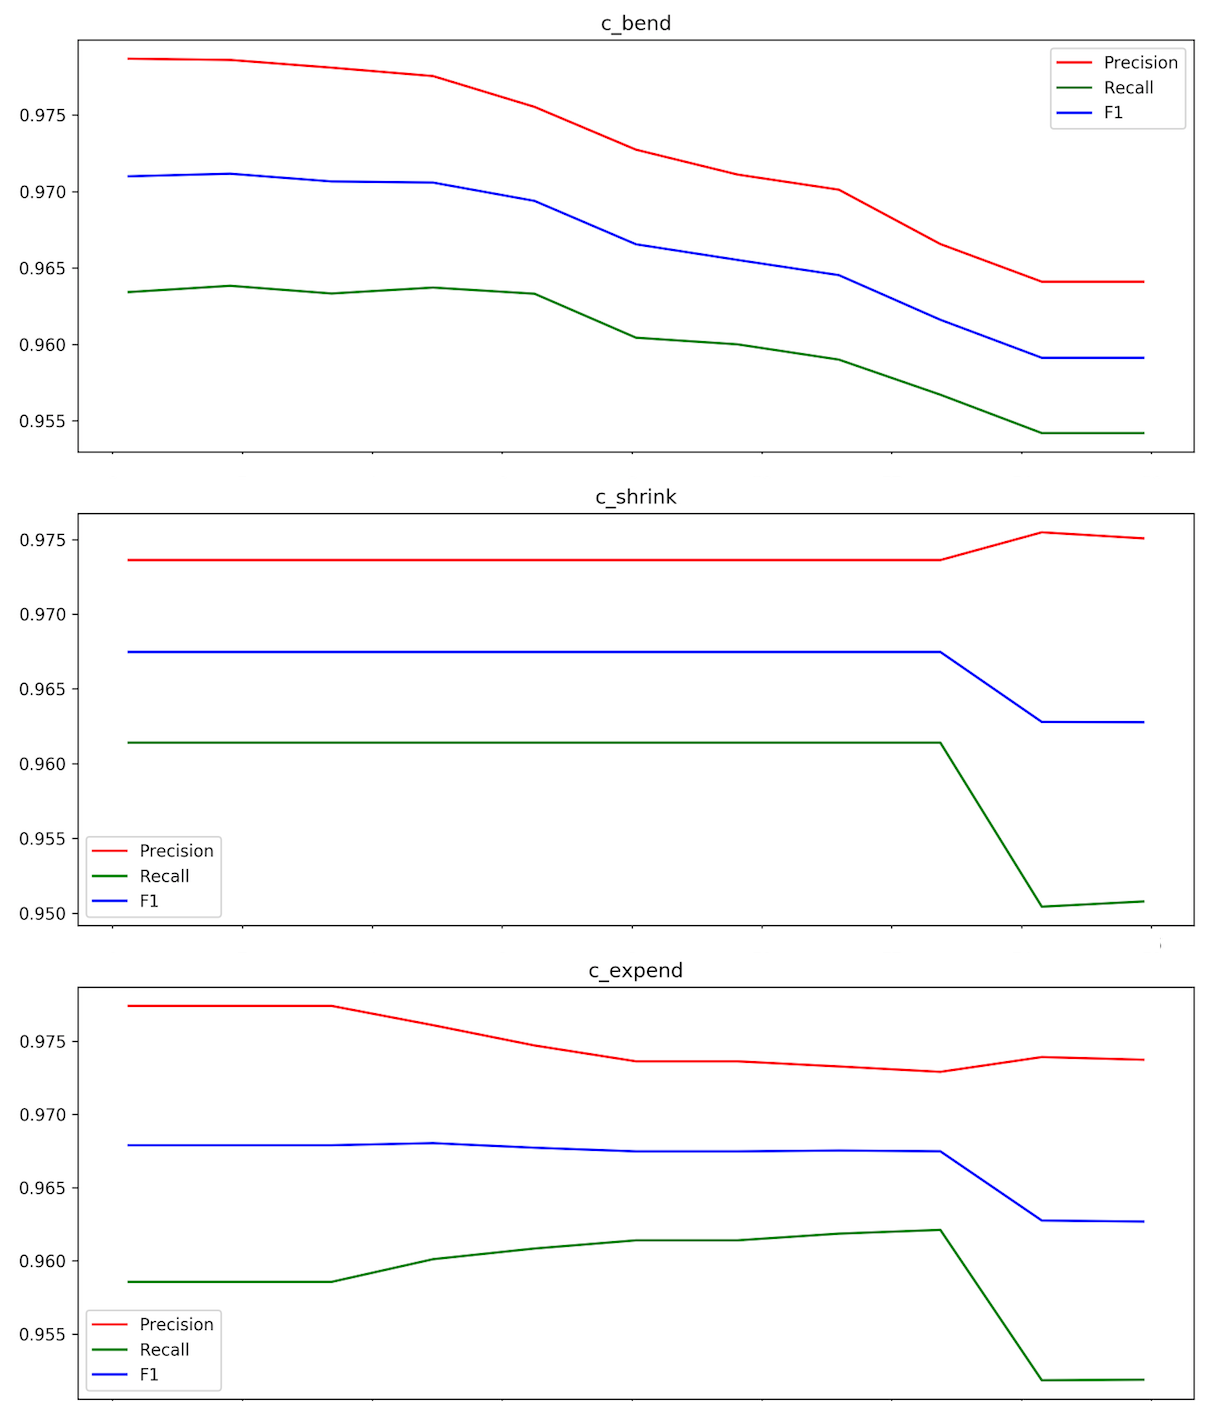
\includegraphics[width=0.85\textwidth]{Figures/prf.png}
    \caption[Parameters Evaluation]{Detail comparison on $c_{bend}$, $c_{shrink}$ and $c_{expand}$. Where red line represent Recall, green line represent Precision and blue line represent F1. We generate these based on equations from Recall (6.2), Precision (6.1), F1 (6.3).}
    \label{fig:change_on_recall}
\end{figure}

We have also identified the following limitations of the proposed method: it assumes that an initial ribbon overlaps with the feature in the corresponding orthophoto. 
We have not suggested an approach to determine if a walking path has been removed, or has been completely occluded. Furthermore, we assume \ac{VHR} orthoimagery that has enough resolution to build a model for colors on and off the ribbon. 
The proposed approach finds integer raddii, so thicknesses are all multiples of two. 
We recommend up-sampling images, which will allow the proposed approach to solve for a trajectory with sub-pixel precision. 
Finally, while we do make some assumptions when we select $\MinRadius{}, \MaxRadius{}, \MaxDistance{}$ the method as presented does not impose a prior on expected thickness of ribbons; often this is known and it could be used to generate plausible results for completely occluded ribbons.

We also test our approach in different cities. 
For initial trajectories, we pull the corresponding footway data from overpass-turbo \cite{overpass_turbo}.
Finding map data is challenging since there not exist much \ac{VHR} imagery from public source. 
We use the imagery data form GIS government database and treat it as input map. 
\figref{fig:oxford1} demonstrate plausible result on a sidewalks heavy area, we randomly selected a few from Oxford, OH. 
Row 1 shows that our approach are able to find the precise boundaries under trees or building shadows, with less accuracy around intersection area. 
Except above from row1, row 2 also demonstrate the camouflage with adjacent material. 
We treat the intersection part as overlapping sidewalks, and process them individually. \figref{fig:ny1} and \figref{fig:ny3} show the random samples we select from New York area. 
Predicting is heavier involved in these area since some sidewalks are partially under tree leaves instead of just shadows. 

% \todo[TALK ABOUT OTHER CITY]

% We generated few results from our sample inputs to compare with other methods according to figure \ref{fig:Sample_4_compare} and mathematics feedback from table \ref{table:sample_4}. From above feedback, Grabcut had decent performance with recognized edges for given sidewalk, since it's false positive (Red) in figure \ref{fig:Sample_4_compare} is significantly small. The problem that mentioned in chapter 2 is still the main reason that it's result is less accurate than ours. In row 1, 2, 3, column 1 of figure \ref{fig:Sample_4_compare}, the grabcut is unable to segment sidewalks which under the tree shadows. For the same issue, in column 4, our result indicated that we could successfully recognize and get boundaries from sidewalk. Same with figure \ref{fig:Sample_2_compare}. In row 1, 2, 3, we compared the output from column 1 and column 4, which are the outputs from grabcut and our approach. It's clear that our approach can successfully segment sidewalk when it connects with drive way (column 1), or there's obstacle (column 3) exist, not only for tree shadows. Also, another advantage of our algorithm is that our approach can segment sidewalks from gutters. We believe other methods are not able to recognize gutter under any circumstances. 

\begin{figure}
    \centering
    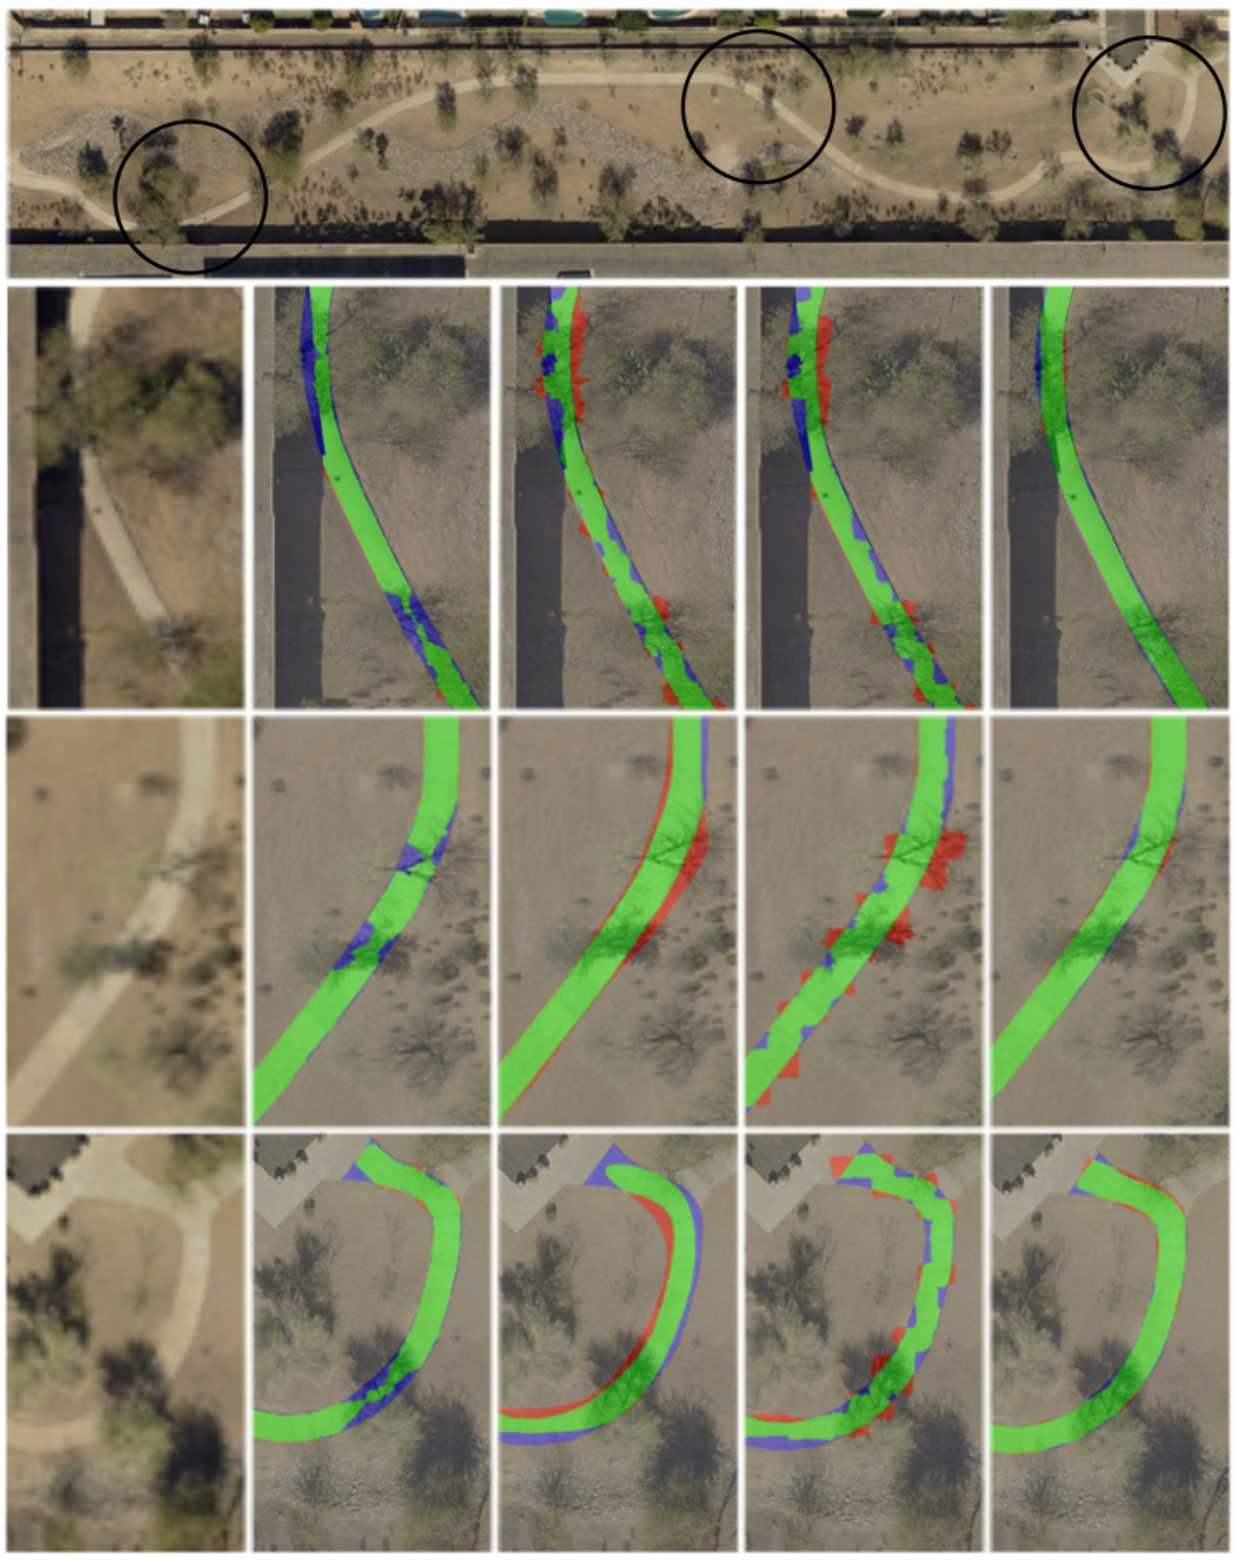
\includegraphics[width=0.9\textwidth]{Figures/4_comparison.pdf}
    \caption[Methods Comparison on Sample Sidewalk 1]{A sample result compared with three different methods and ours. In the order of grabcut, slic, active Contours and ours from left to right. Grabcut is unable to separate the tree shadow from actual sidewalk feature, same with slic and active contours. Our results are more likely to predict the accurate edges under obstacles.}
    \label{fig:Sample_4_compare}
\end{figure}

% \begin{table}[h]
% 	\centering
% 	\begin{tabular}{ | c | c | c | c | } 
% 		\hline
% 		Methods	& TP-FP\% & TP\% & FP\% \\
% 		\hline
% 		Grabcut			& 86.10\% & 87.69\% & 1.82\% \\
% 		\hline
% 		Slic			& 73.90\% & 83.88\% & 11.90\% \\
% 		\hline
% 		Active Contour	& 75.70\% & 86.63\% & 12.63\% \\
% 		\hline
% 		Ours            & 93.48\% & 96.06\% & 2.69\% \\
% 		\hline
% 	\end{tabular}
% 	\caption{Mathematics result comparison between our result and others from figure \ref{fig:Sample_4_compare}}
% 	\label{table:sample_4}	
% \end{table}

\begin{figure}
    \centering
    \includegraphics[width=0.78\textwidth]{Figures/sample_sidewalk_1.png}
    \caption[Methods Comparison on Sample Sidewalk 2]{A sample results compared with three different methods and ours. In the order of active Contours, grabcut, slic, ours from left to right. Which shows samples of separating drive way and gutters.}
    \label{fig:Sample_2_compare}
\end{figure}

\begin{figure}
    \centering
    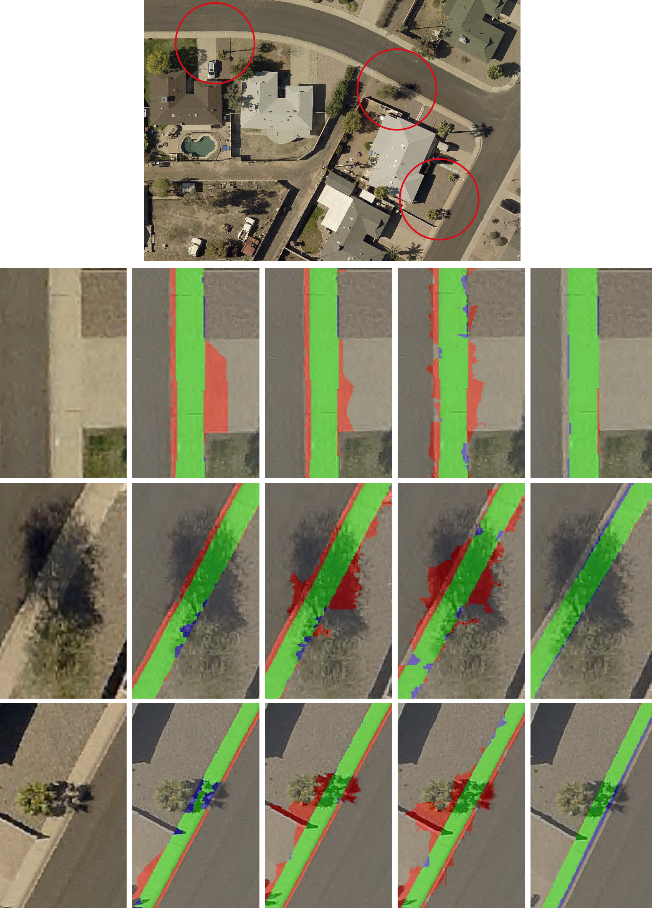
\includegraphics[width=0.86\textwidth]{Figures/2_comparison_needed.png}
    \caption[Methods Comparison on Sample Sidewalk 3]{A sample results compared with three different methods and ours. In the order of grabcut, slic, active Contours, ours from left to right. Which shows samples of separating drive way and gutters.}
    \label{fig:Sample_3_compare}
\end{figure}



\begin{figure}
    \centering
    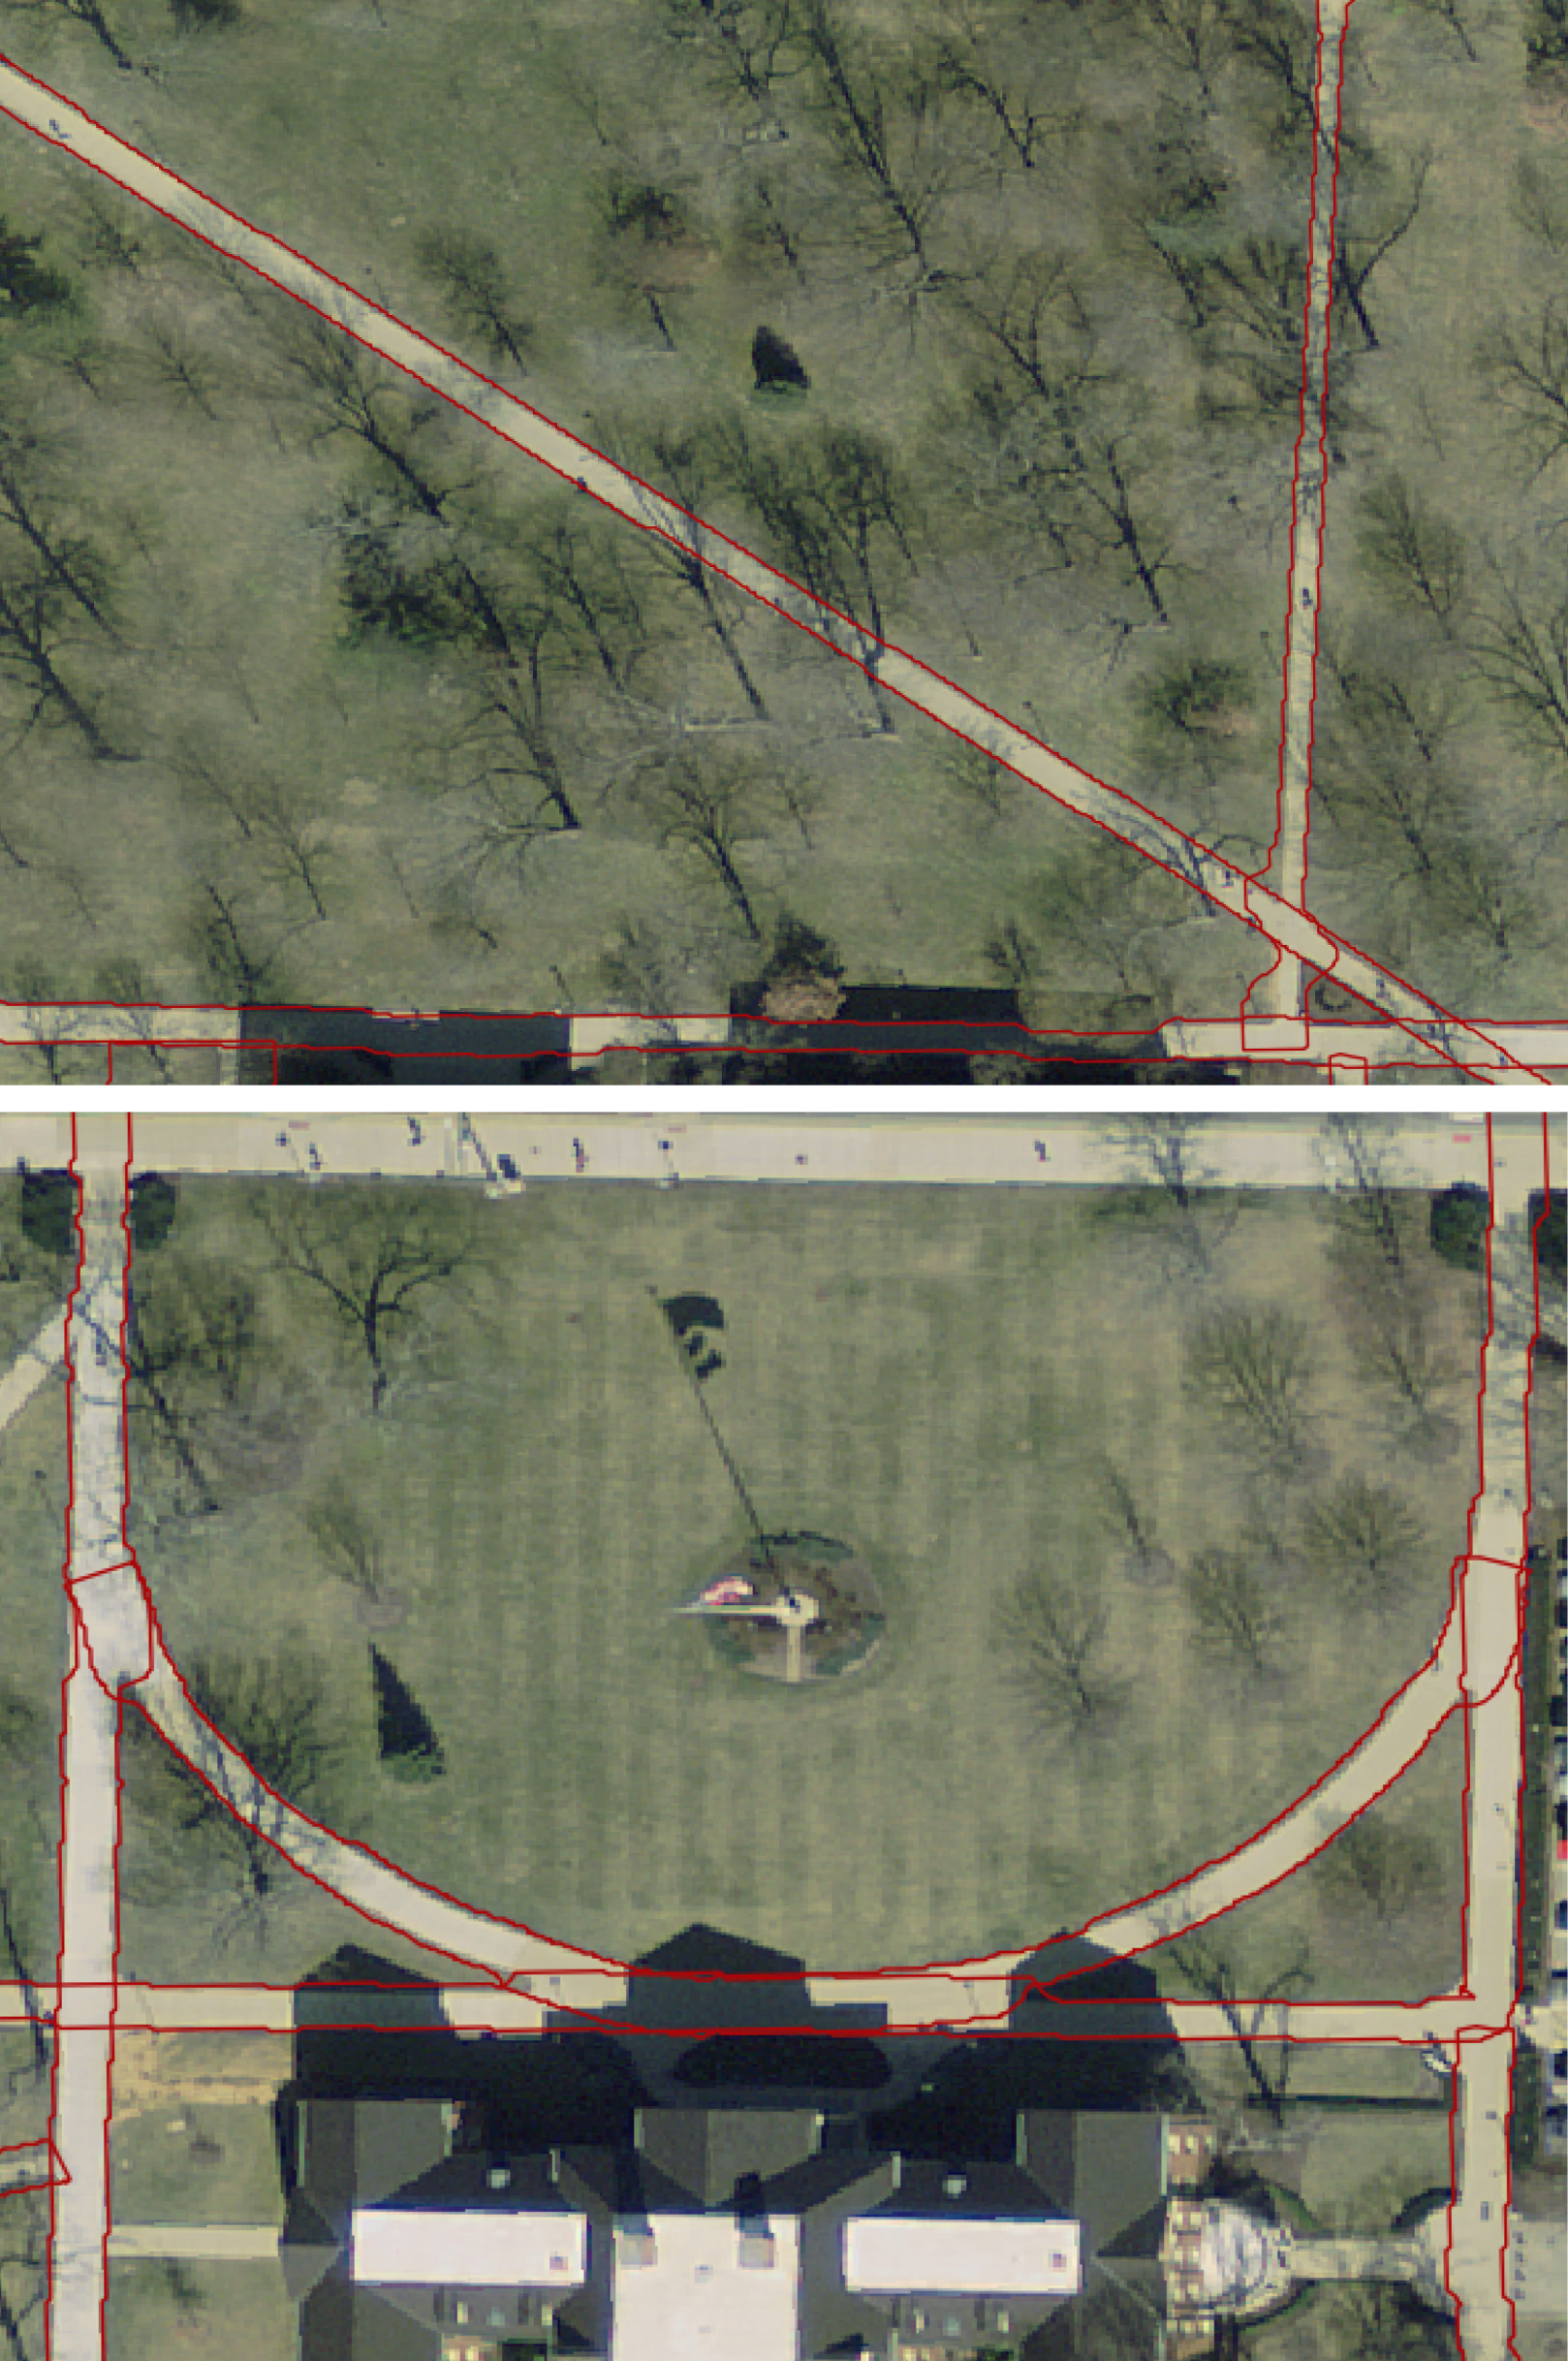
\includegraphics[width=0.8\textwidth]{Figures/Oxford_success_complex.png}
    \caption[Sample Sidewalk 3]{Demonstration on sample sidewalks with our approach. We use Oxford Area that include more complex sidewalks. It shows that given samples are able to separate trees, building shadows and camouflage with adjacent materials.}
    \label{fig:oxford1}
\end{figure}

\begin{figure}
    \centering
    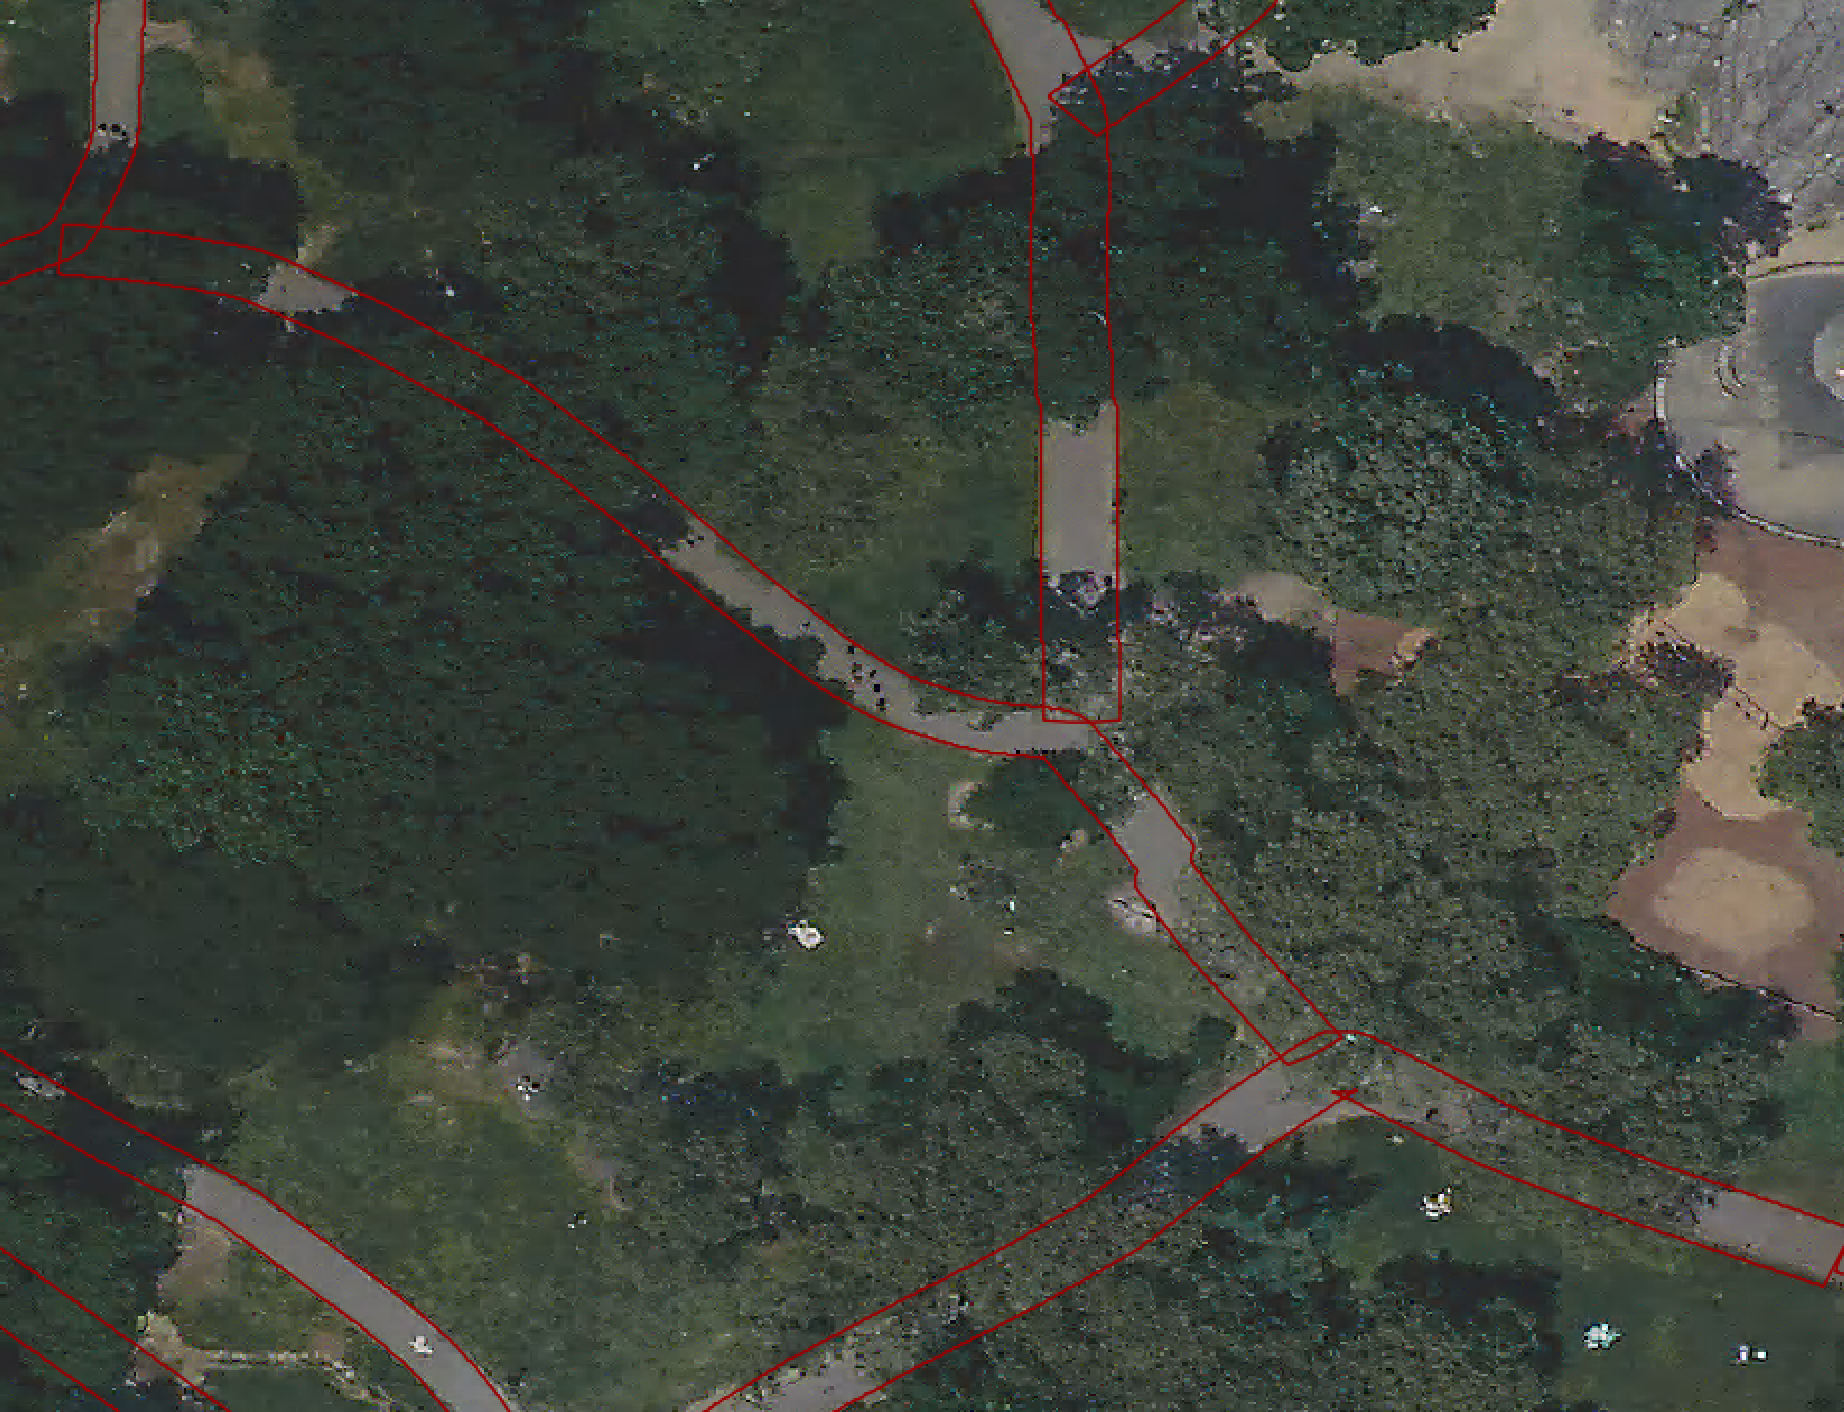
\includegraphics[width=\textwidth]{Figures/ny1.png}
    \caption[Sample Sidewalk 4]{Demonstration on sample sidewalks with our approach. We use New York area that include more complex sidewalks. Our approach is able to separate tree shadows and obstacles. It also has a decent performance on predicating boundaries on partial sidewalks that are fully covered by tree leaves.}
    \label{fig:ny1}
\end{figure}

% \begin{figure}
%     \centering
%     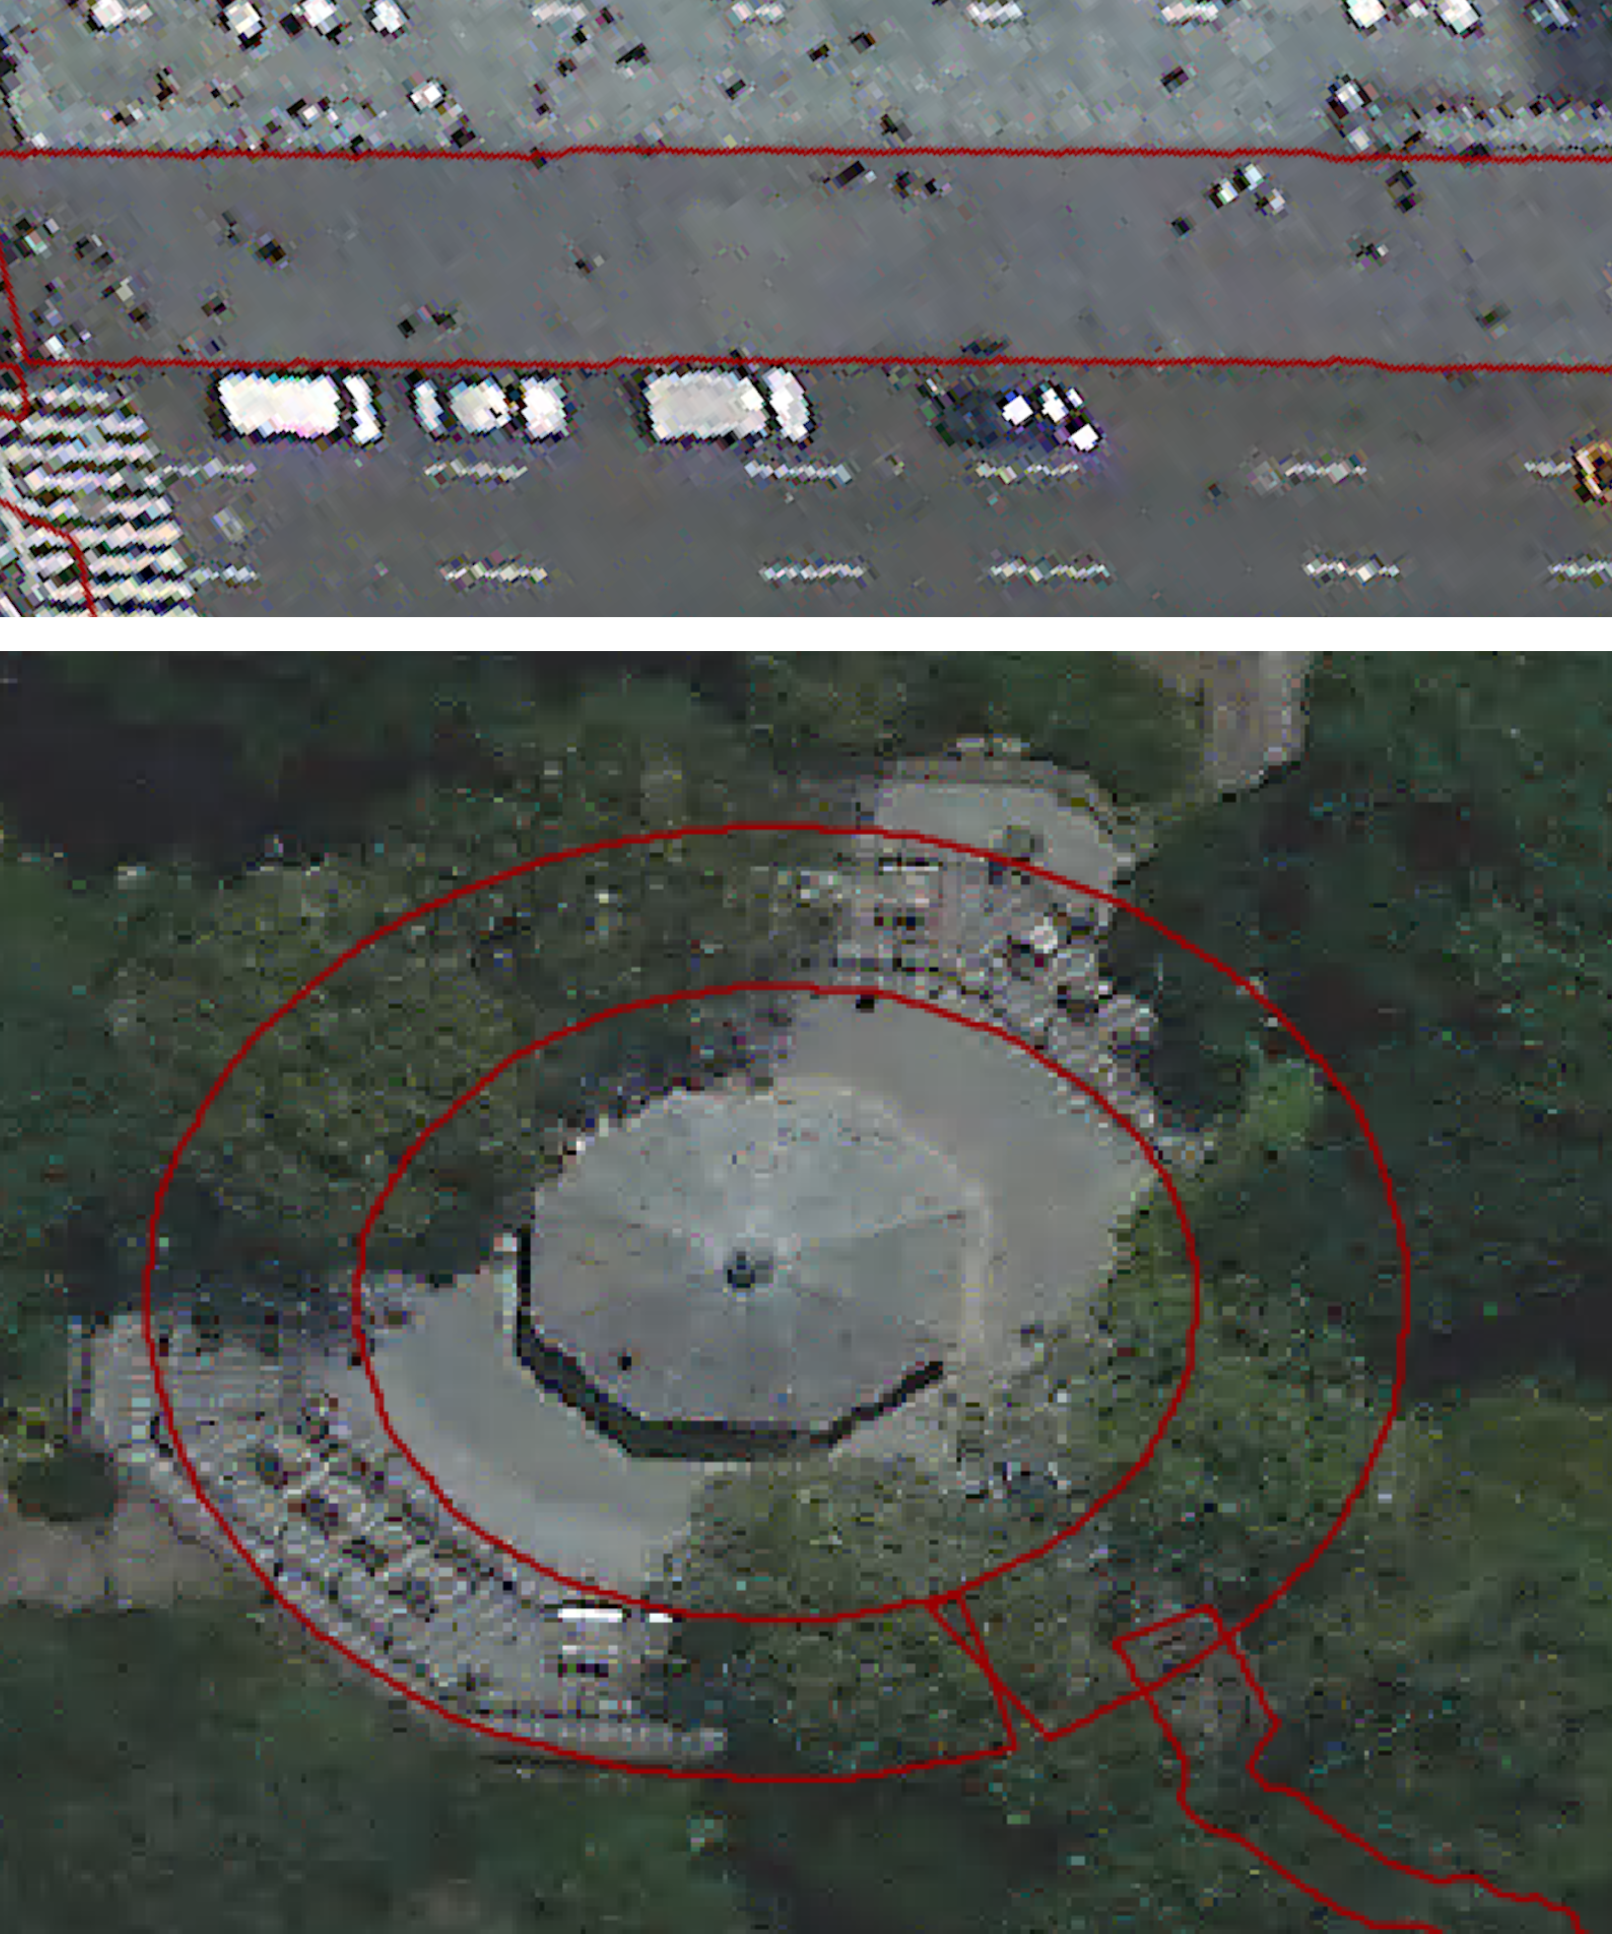
\includegraphics[width=\textwidth]{Figures/ny2.png}
%     \caption[Sample Sidewalk 5]{Demonstration on sample sidewalks with our approach. We use sidewalks that are random selected from New York area. Row 1 shows a thicker sidewalk that camouflage with adjacent road and street. Row 2 shows complex sidewalk texture with irregular shape.}
%     \label{fig:ny2}
% \end{figure}

\begin{figure}
    \centering
    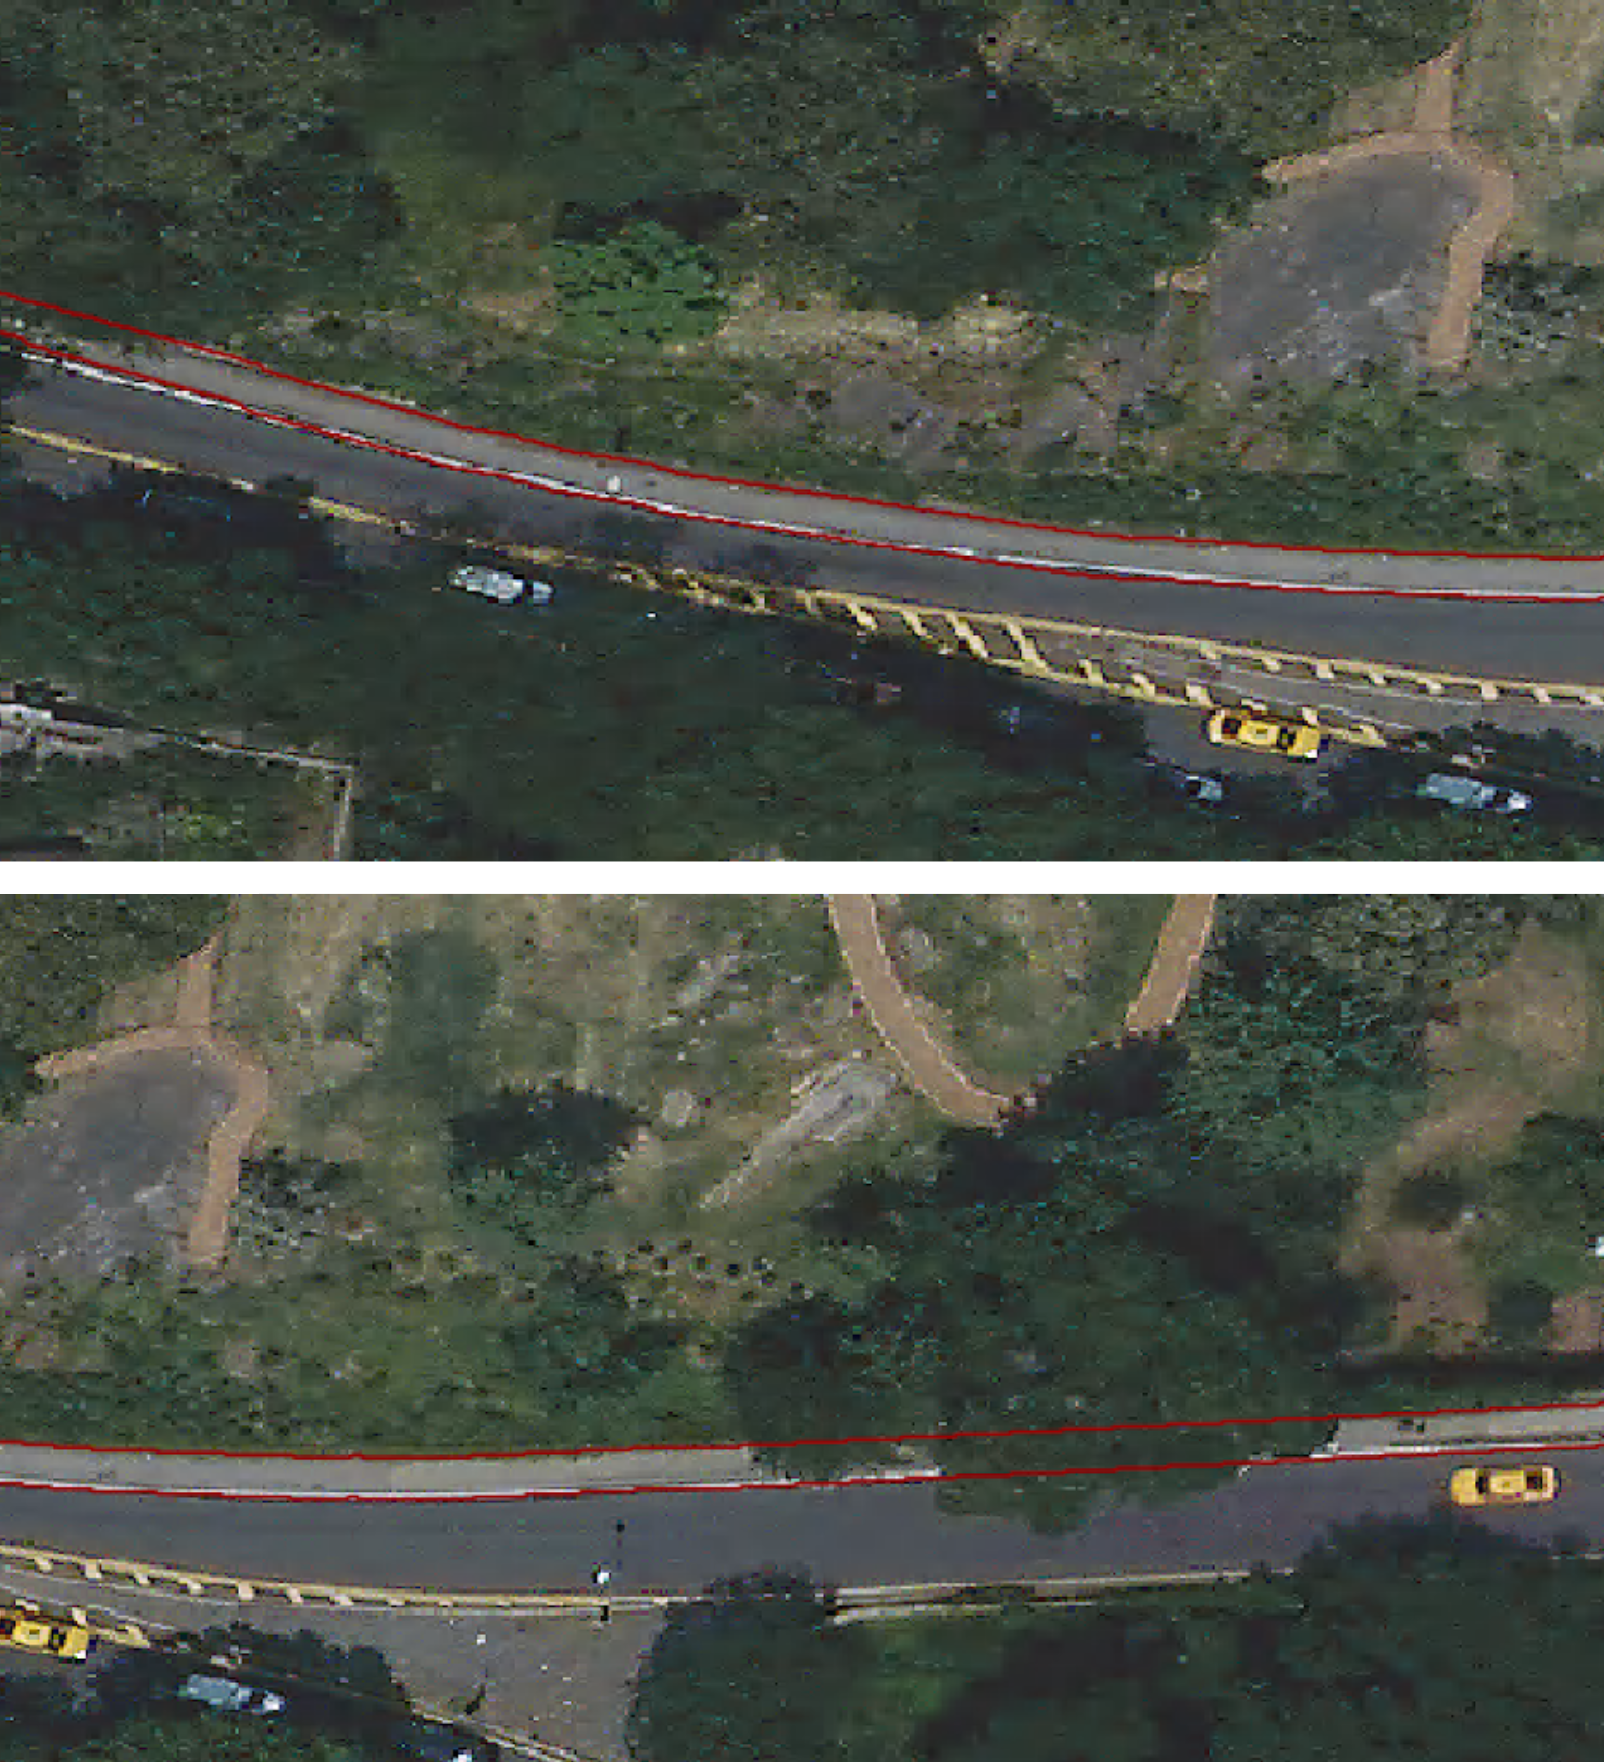
\includegraphics[width=\textwidth]{Figures/ny3.png}
    \caption[Sample Sidewalk 6]{Demonstration on sample sidewalks with our approach. It shows a continues site but we separate it due to it's length. Our approach did recognized the sidewalk part under the tree top and predict it's precise boundaries.}
    \label{fig:ny3}
\end{figure}

